
\documentclass{article}
\usepackage{caption} % do not load that twice
\usepackage{subcaption} % do not load that twice
\usepackage{float}
\usepackage{geometry}
%\usepackage{color} TikZ already loads the newer xcolor
\usepackage{tikz}
\usetikzlibrary{arrows,automata,positioning}
\tikzset{%
    >=stealth,
    place/.style={circle,thick,draw=blue!75,fill=blue!20,minimum size=10mm},
    every label/.style={red},
    every node/.style={scale=.6},
    sh2w/.style={shift={(-0.7,0)}},
    sh2nw/.style={shift={(-0.7,0.5)}},
    sh2ne/.style={shift={(0.7,0.5)}},
    sh2sw/.style={shift={(-0.7,-0.5)}},
    sh2se/.style={shift={(0.7,-0.5)}},
    h2n/.style={shift={(0,1.1)}},
    h2s/.style={shift={(0,-1.1)}},
    h2se/.style={shift={(0.5,-1.1)}},
    rc/.style={rounded corners=2mm} 
}
\usepackage{mathtools}
\newsavebox{\tempbox}

\begin{document}
    \sbox{\tempbox}{%
            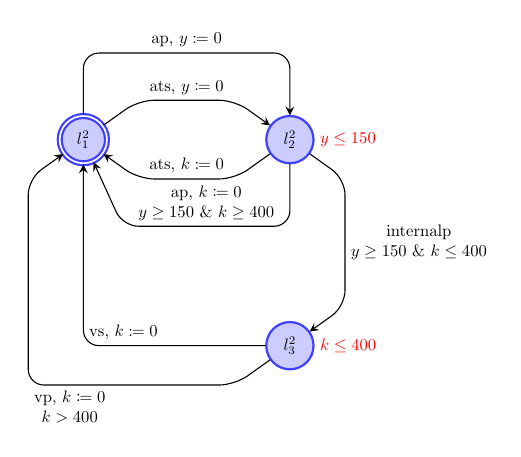
\begin{tikzpicture}[->,node distance=2cm]
            \node [accepting, place] (l2-1) {$l_1^2$};
            \node [place,right= of l2-1,label={0:$y\le150$}] (l2-2) {$l_2^2$};
            \node [place,below= of l2-2,label={0:$k\le400$}] (l2-3) {$l_3^2$};
            %%%%%
            \draw[rc] (l2-1) -- ([sh2ne]l2-1.center) -- node[above]
            {ats, $y\coloneqq 0$}  ([sh2nw]l2-2.center) -- (l2-2);
            \draw[rc] (l2-1) -- ([h2n]l2-1.center) -- node[above]
            {ap, $y\coloneqq 0$}  ([h2n]l2-2.center) -- (l2-2);
            \draw[rc] (l2-2) -- ([sh2sw]l2-2.center) -- node[above]
            {ats, $k\coloneqq 0$}  ([sh2se]l2-1.center) -- (l2-1);
            \draw[rc] (l2-2) -- ([h2s]l2-2.center) -- node[above,align=center]
            {ap, $k\coloneqq 0$\\$y\ge150 \text{ \& } k\ge400$}  ([h2se]l2-1.center) -- (l2-1);
            \draw[rc] (l2-2) -- ([sh2se]l2-2.center) -- node[right,align=center]
            {internalp\\ $y\ge150 \text{ \& } k\le400$}  ([sh2ne]l2-3.center) -- (l2-3);
            \draw[rc] (l2-3) -- ([sh2w]l2-3.center) -| node[above right]
            {vs, $k\coloneqq 0$} (l2-1);
            \draw[rc] (l2-3) -- ([sh2sw]l2-3.center) -| node[below right,align=center]
            {vp, $k\coloneqq 0$\\$k>400$} ([sh2sw]l2-1.center) -- (l2-1);
            \end{tikzpicture}%
    }%

    \begin{figure}[H]
        \centering
        \begin{subfigure}[b]{.45\textwidth}
            \centering
            \vbox to\ht\tempbox{\vfil
            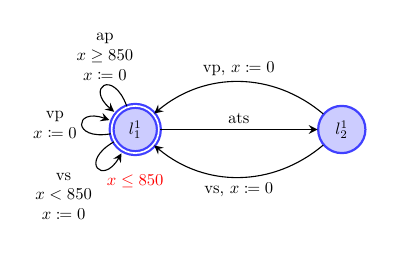
\begin{tikzpicture}[->,node distance=2cm,bend angle=40]
            \node [accepting, place,label={[label distance=.3cm]270:$x\le850$}] (l1-1) {$l_1^1$};
            \node [place,right= of l1-1] (l1-2) {$l_2^1$};
            %%%%%
            \path (l1-1) edge [in=160,out=190,loop,align=center] node[left]{vp\\$x\coloneqq0$} (l1-1)
            edge [in=240,out=210,loop,align=center] node[below left]{vs\\
                $x < 850$\\$x\coloneqq 0$} (l1-1)
            edge [in=140, out=110,loop,align=center] node[above]{ap\\$x \ge 850$
                \\$x\coloneqq0$} (l1-1)
            (l1-1) edge node[above]{ats} (l1-2)
            (l1-2) edge [bend right] node[above]{vp, $x\coloneqq0$} (l1-1)
            edge [bend left] node[below]{vs, $x\coloneqq0$} (l1-1);
            \end{tikzpicture}\vfil}
            \caption{LRI}\label{fig:p1}
        \end{subfigure}\hfil
        \begin{subfigure}[b]{.45\textwidth}
            \centering
            \usebox\tempbox
            \caption{AVI-URI}\label{fig:p2}
        \end{subfigure}

        \begin{subfigure}[c]{.45\textwidth}
            \centering
            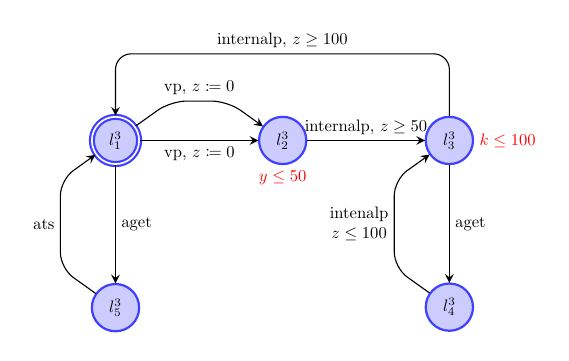
\begin{tikzpicture}[->,node distance=1.5cm]
            \node [accepting, place] (l3-1)  {$l_1^3$};
            \node [place,right= of l3-1,label={270:$y\le50$}] (l3-2) {$l_2^3$};
            \node [place,right= of l3-2,label={0:$k\le100$}] (l3-3) {$l_3^3$};
            \node [place,below= of l3-3] (l3-4) {$l_4^3$};
            \node [place,below= of l3-1] (l3-5) {$l_5^3$};
            %%%%%
            \draw[rc] (l3-3) -- ([h2n]l3-3.center) -- node[above]
            {internalp, $z\ge100$}  ([h2n]l3-1.center) -- (l3-1);
            \draw[rc] (l3-1) -- ([sh2ne]l3-1.center) -- node[above]{vp, $z\coloneqq 0$}
            ([sh2nw]l3-2.center) -- (l3-2);
            \draw[rc] (l3-5) -- ([sh2nw]l3-5.center) -- node[left]{ats}
            ([sh2sw]l3-1.center) -- (l3-1);
            \draw[rc] (l3-4) -- ([sh2nw]l3-4.center) -- node[left,align=center]
            {intenalp\\ $z\le100$}  ([sh2sw]l3-3.center) -- (l3-3);
            \path (l3-1) edge node[below]{vp, $z\coloneqq 0$} (l3-2)
            edge node[right]{aget} (l3-5)
            (l3-2) edge node[above]{internalp, $z\ge50$} (l3-3)
            (l3-3) edge node[right]{aget} (l3-4);
            \end{tikzpicture}
            \caption{PVARP}\label{fig:p3}
        \end{subfigure}\hfil
        \begin{subfigure}[c]{.45\textwidth}
            \centering
            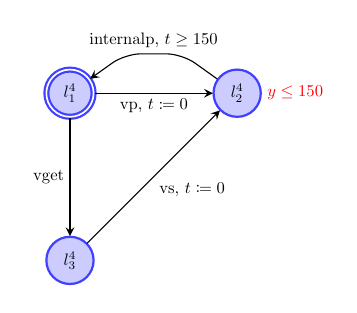
\begin{tikzpicture}[->,node distance=1.5cm]
            \node [accepting, place] (l4-1)  {$l_1^4$};
            \node [place,right= of l4-1,label={0:$y\le150$}] (l4-2) {$l_2^4$};
            \node [place,below= of l4-1] (l4-3) {$l_3^4$};
            %%%%%
            \draw[rc] (l4-2) -- ([sh2nw]l4-2.center) -- node[above]
            {internalp, $t\ge150$}  ([sh2ne]l4-1.center) -- (l4-1);
            \path (l4-1) edge node[left]{vget} (l4-3)
            edge node[below]{vp, $t\coloneqq 0$} (l4-2)
            (l4-3) edge node[below right]{vs, $t\coloneqq 0$} (l4-2);
            \end{tikzpicture}
            \caption{VRP}\label{fig:p4}
        \end{subfigure}
        \caption{Pacemaker system modeled in BIP}\label{fig:paceg}
    \end{figure}
\end{document}
